\begin{apendicesenv}

\chapter{Supplementary figures}\label{ap:supplementary}

This appendix collects the supporting analyses referred to in the Results and Discussion chapters. They are secondary to the main
argument but are reported here so that the results can be checked in full: the pattern separation of the mGCs resolved by input
similarity (Figure~\ref{fig:pattern_separation_similarity}), the population sparsity measured with the Hoyer index as a
cross-validation of the Gini results (Figure~\ref{fig:sparsity_hoyer}), the orthogonalization of the mGC output
(Figure~\ref{fig:mgc_orthogonalization}), the population sparsity immediately before and after direct iGC activation for each
EC$\to$iGC connection probability (Figure~\ref{fig:opto_sparsity}), and the post-pulse population rate and power spectrum of every
cell type (Figure~\ref{fig:frequency_spectra}).

\begin{figure}[H]
    \centering
    \caption{Pattern separation of the mature granule cells resolved by input similarity. Each curve shows the pattern separation
        degree $\mathcal{S}_D$ of the mGC population as a function of the similarity between the input patterns, for the control
        network without neurogenesis (black dashed line) and for neurogenesis networks at representative EC$\to$iGC connection
        probabilities. Each point is the mean over the 30 pattern sets and the shaded band shows the standard error of the mean.
        The gray dashed line marks $\mathcal{S}_D = 1$, above which the output patterns are more distinct than their inputs.
        Separation is strongest for the most similar (most overlapping) inputs, and every neurogenesis network separates better
        than the control across the whole similarity range.}

    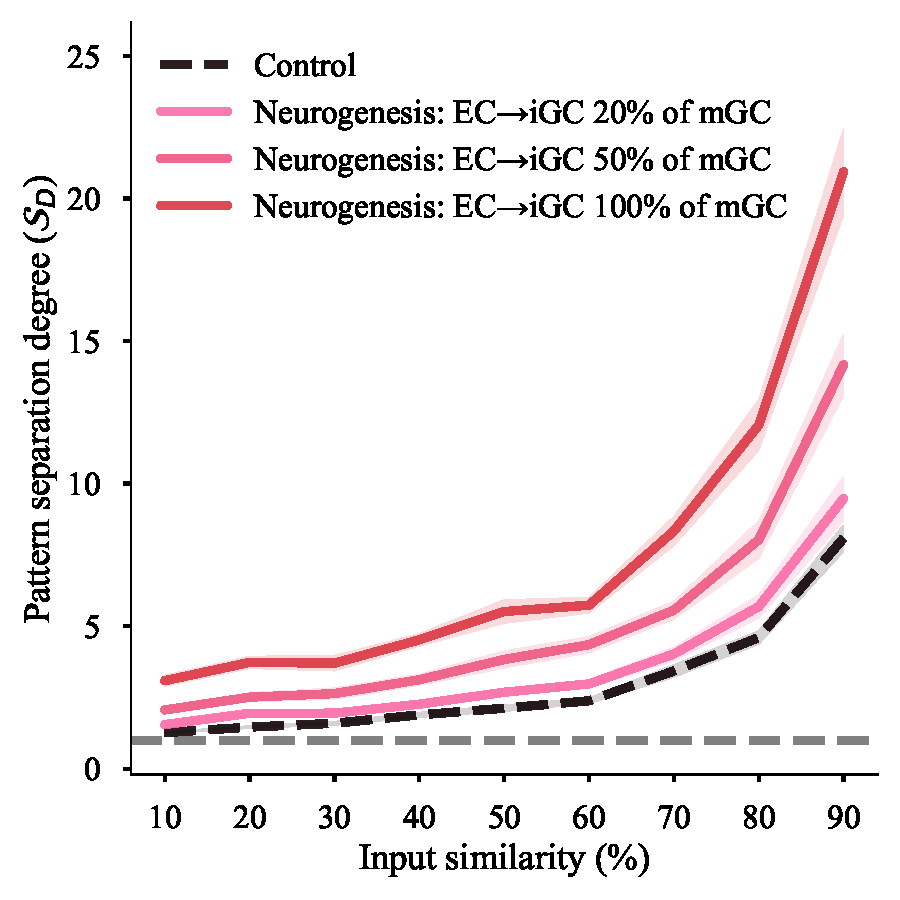
\includegraphics[width=0.8\textwidth]{figures/supplementary/pattern_separation.pdf}%
\label{fig:pattern_separation_similarity}
\end{figure}

\begin{figure}[H]
    \centering
    \caption{Population sparsity measured with the Hoyer index, as a cross-validation of the Gini results reported in the Results
        chapter. Each panel shows the Hoyer sparsity of one population, the whole granule-cell population (All GC), the mature
        granule cells (mGC), the immature granule cells (iGC) and the pyramidal CA3 cells (pCA3), as a function of the
        EC$\to$iGC connection probability; the shaded bands show the standard error of the mean and the dashed line marks the
        control network without neurogenesis (absent for the iGC panel, which has no counterpart in the control). As with the
        Gini index, the sparsity of the All GC, mGC and pCA3 populations rises with the EC$\to$iGC connection probability and
        stays above the control, whereas the iGC population becomes less sparse.}

    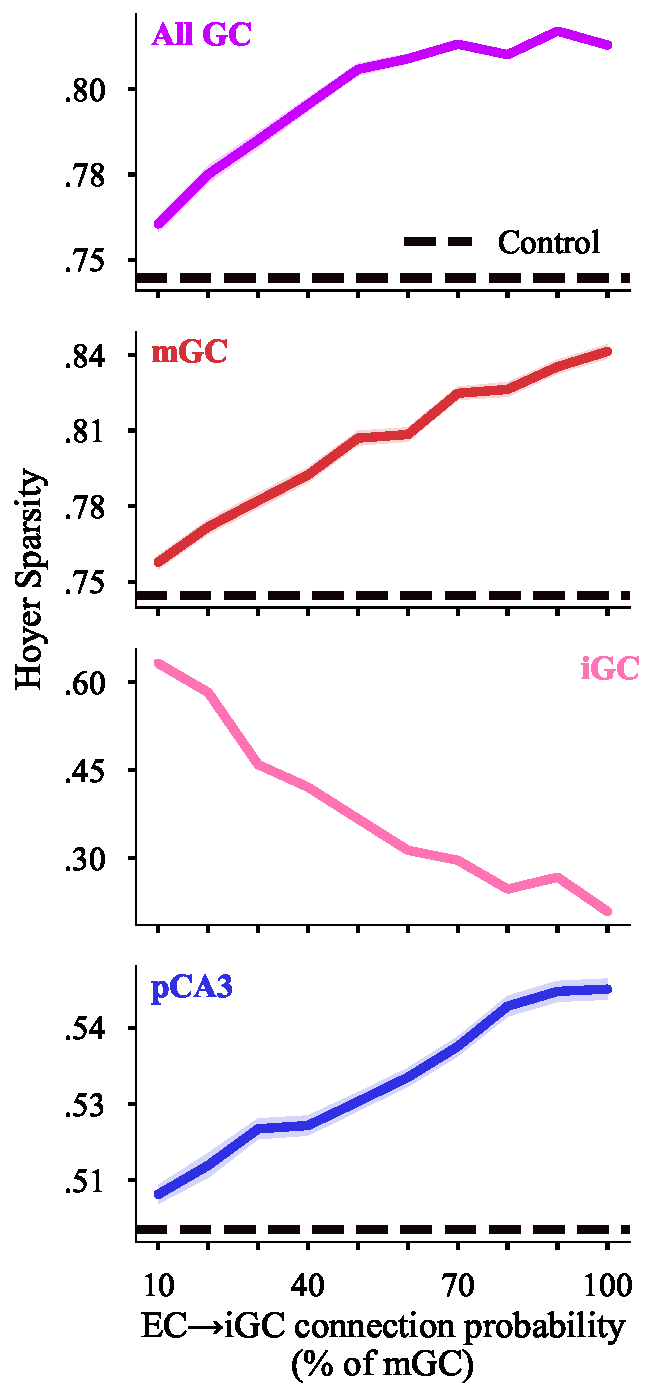
\includegraphics[width=0.45\textwidth]{figures/supplementary/sparsity_hoyer.pdf}%
\label{fig:sparsity_hoyer}
\end{figure}

\begin{figure}[H]
    \centering
    \caption{Orthogonalization of the mature granule-cell output as a function of the EC$\to$iGC connection probability. The
        curve shows the orthogonalization degree $\mathcal{O}_D$ of the mGC population, taken as the ratio of the output to the
        input orthogonalization ($\mathcal{O}^{(out)}/\mathcal{O}^{(in)}$); the shaded band shows the standard error of the mean
        and the dashed line marks the control network without neurogenesis. The orthogonalization rises with the EC$\to$iGC
        connection probability, indicating that the mGC outputs become increasingly decorrelated as neurogenesis increases,
        beyond what the reduction in the number of active
        cells alone would produce.}

    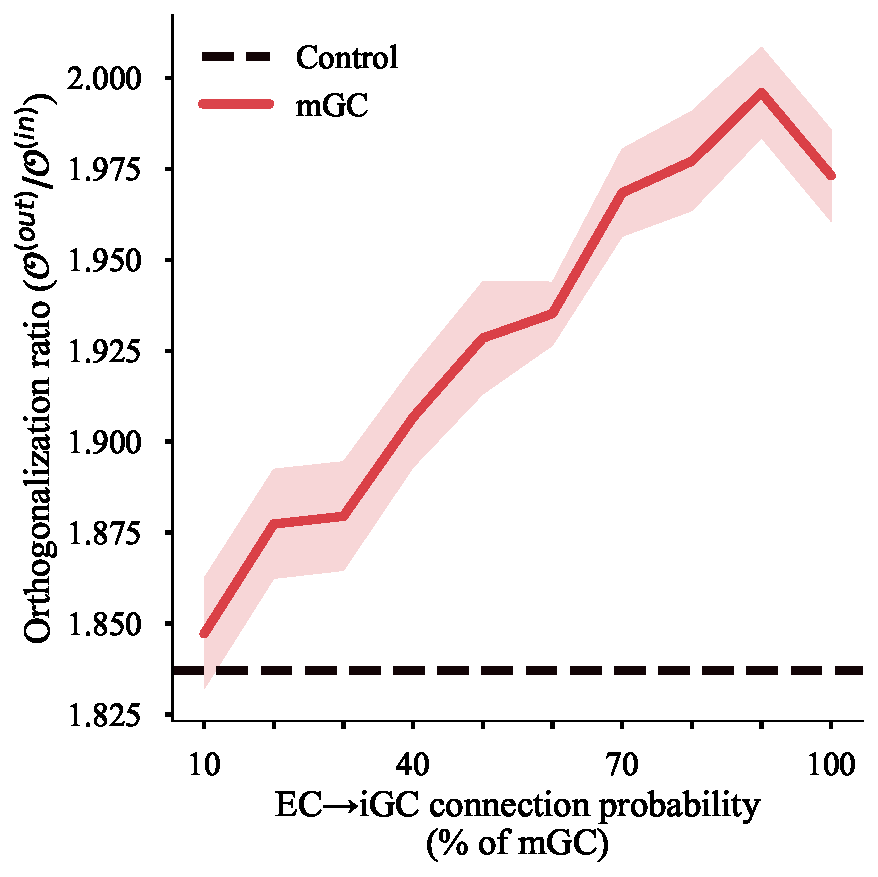
\includegraphics[width=0.7\textwidth]{figures/supplementary/mgc_orthogonalization.pdf}%
\label{fig:mgc_orthogonalization}
\end{figure}

\clearpage
\begin{figure}[H]
    \centering
    \caption{Population sparsity (Gini index) immediately before and after direct iGC activation, for every EC$\to$iGC
        connection probability. Each panel corresponds to one EC$\to$iGC connection probability, given in the panel title as a
        percentage of the EC$\to$mGC value (10\%--100\%), and compares the Gini index of the mGC, iGC, combined granule-cell
        (all GC) and pCA3 populations in the \SI{50}{\milli\second} windows immediately before (pre) and after (post) the
        depolarizing pulse, pooled over all runs. Bars show the mean across runs.
        The result of the paired Wilcoxon signed-rank test between the pre and post values is indicated above each pair (ns, not
        significant; {*}~$p < 0.05$; {**}~$p < 0.01$; {***}~$p < 0.001$).}

    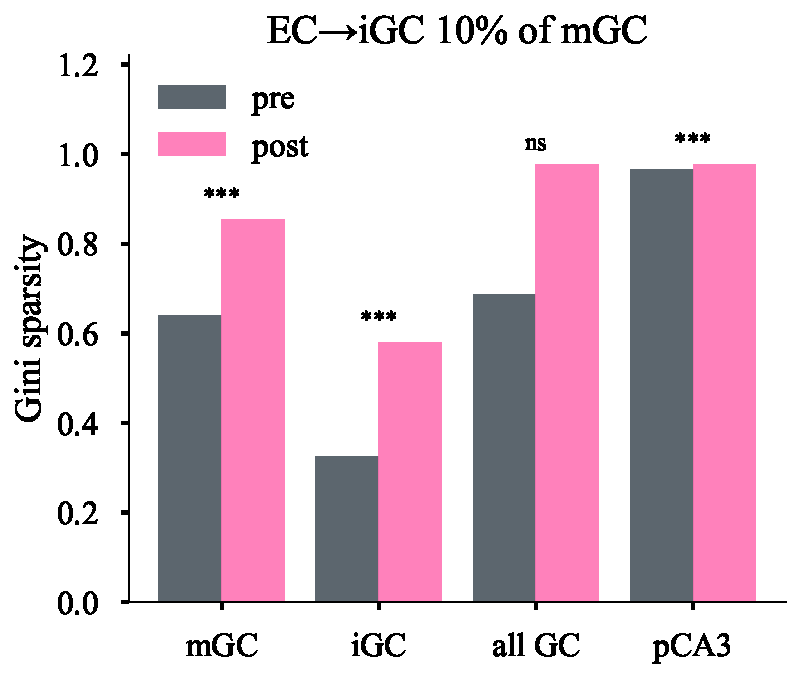
\includegraphics[width=0.31\textwidth]{figures/supplementary/opto_sparsity_neurogenesis_0.1.pdf}\hfill
    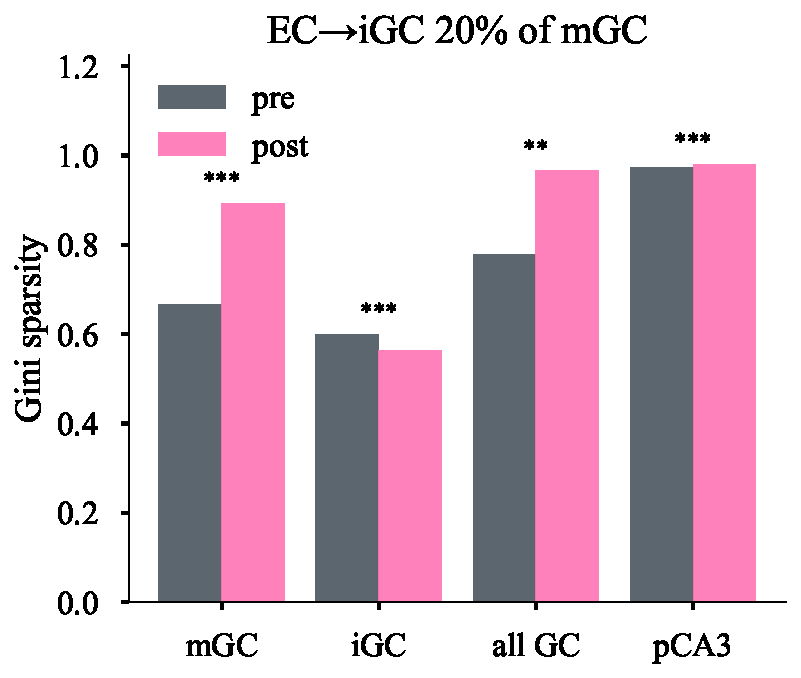
\includegraphics[width=0.31\textwidth]{figures/supplementary/opto_sparsity_neurogenesis_0.2.pdf}\hfill
    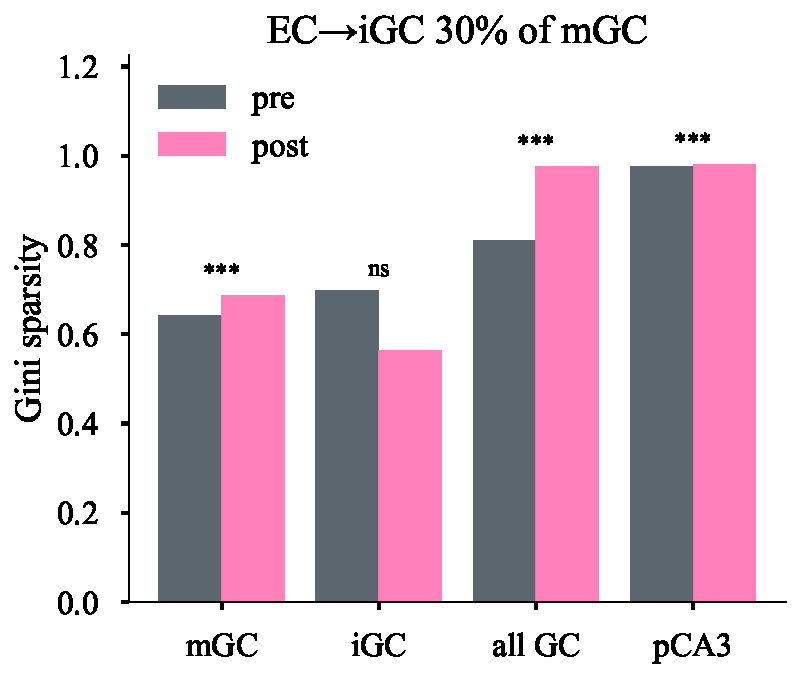
\includegraphics[width=0.31\textwidth]{figures/supplementary/opto_sparsity_neurogenesis_0.3.pdf}

    \medskip

    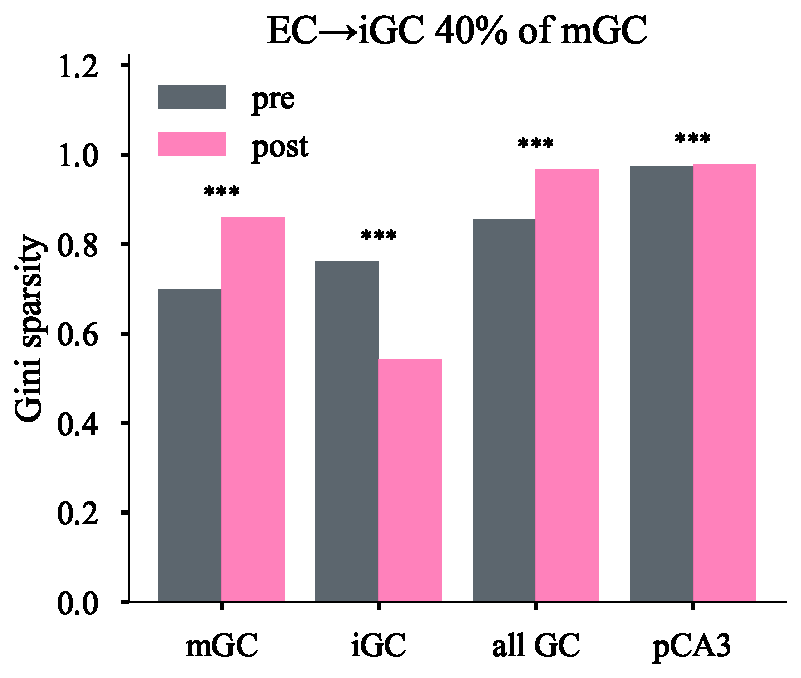
\includegraphics[width=0.31\textwidth]{figures/supplementary/opto_sparsity_neurogenesis_0.4.pdf}\hfill
    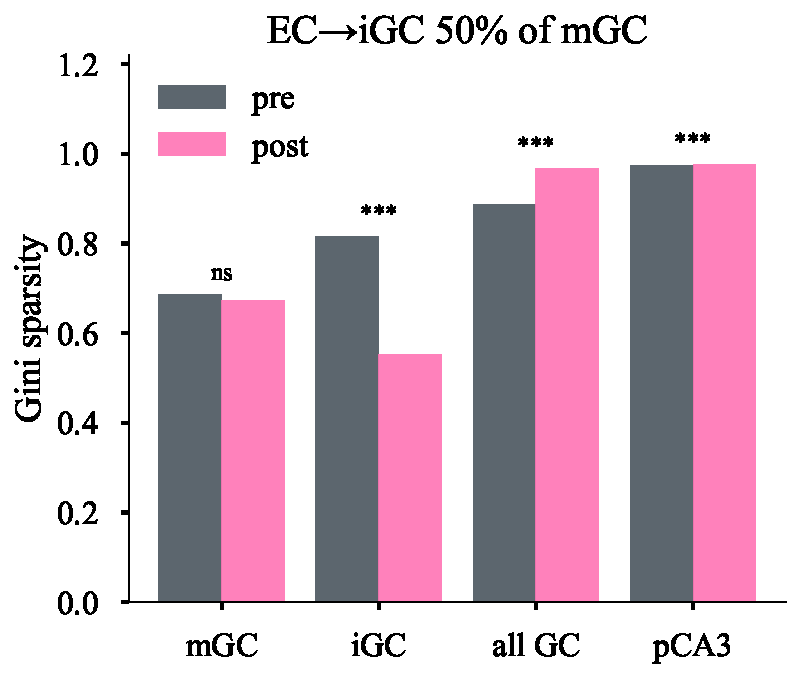
\includegraphics[width=0.31\textwidth]{figures/supplementary/opto_sparsity_neurogenesis_0.5.pdf}\hfill
    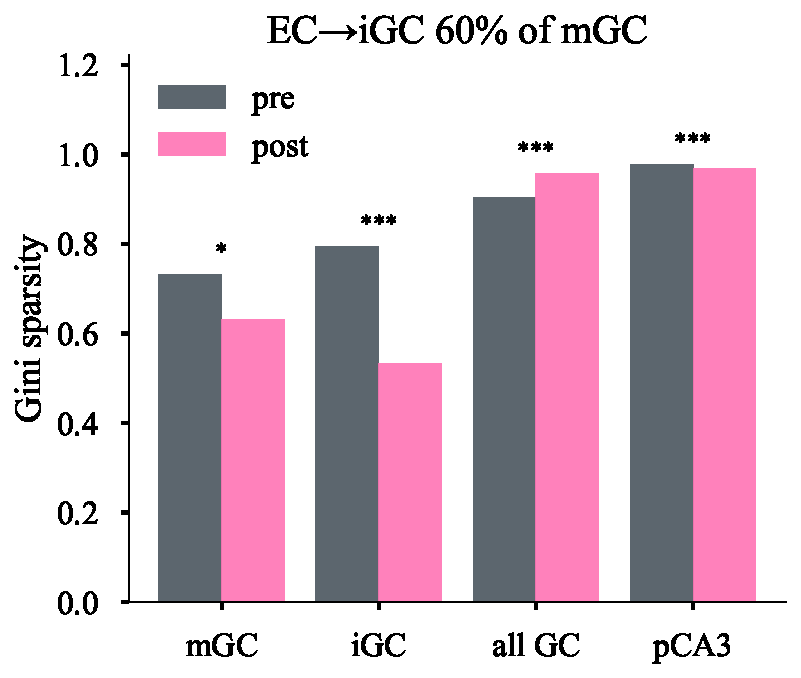
\includegraphics[width=0.31\textwidth]{figures/supplementary/opto_sparsity_neurogenesis_0.6.pdf}

    \medskip

    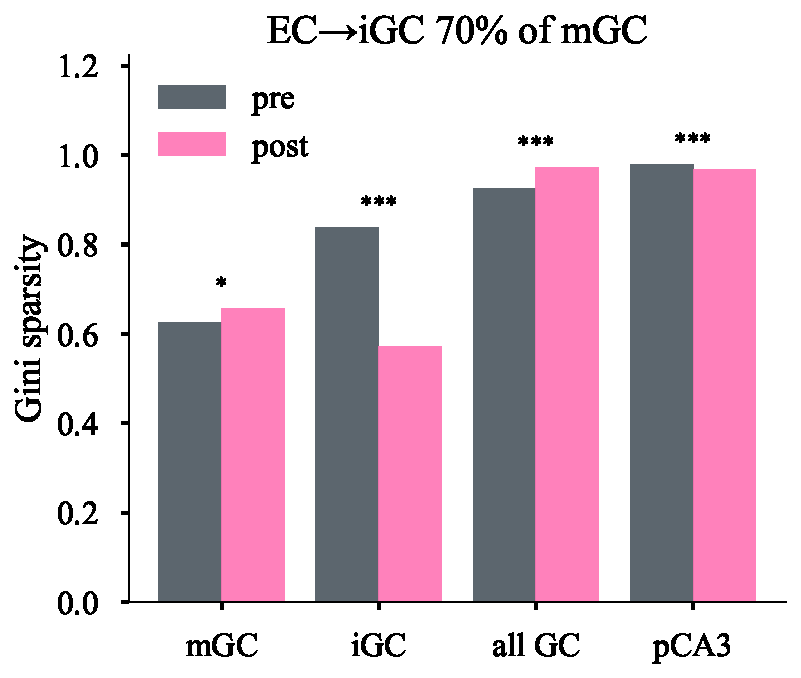
\includegraphics[width=0.31\textwidth]{figures/supplementary/opto_sparsity_neurogenesis_0.7.pdf}\hfill
    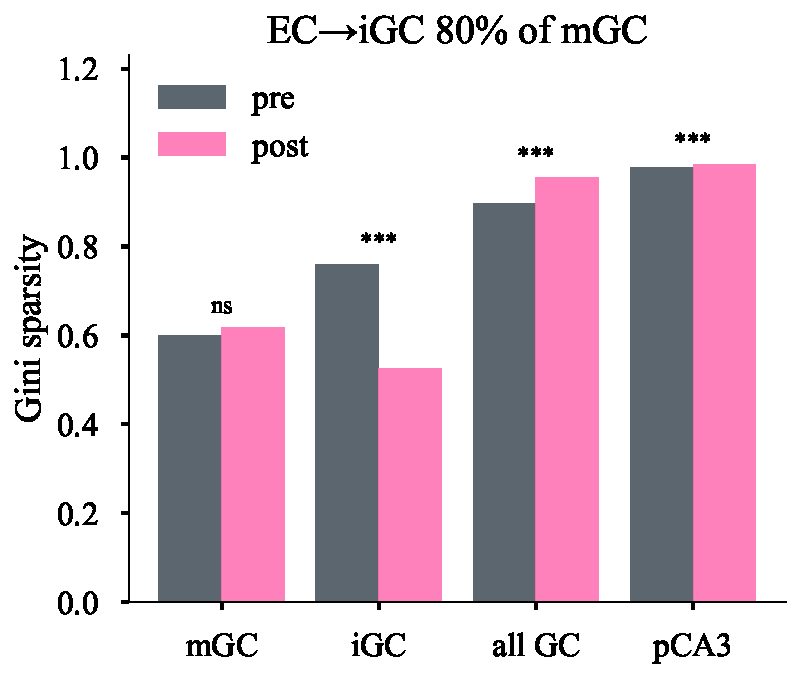
\includegraphics[width=0.31\textwidth]{figures/supplementary/opto_sparsity_neurogenesis_0.8.pdf}\hfill
    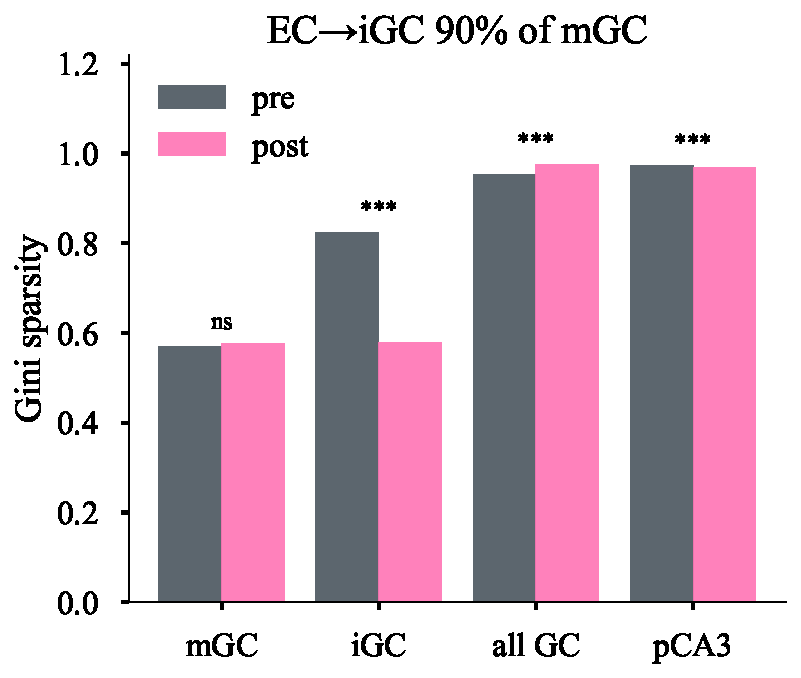
\includegraphics[width=0.31\textwidth]{figures/supplementary/opto_sparsity_neurogenesis_0.9.pdf}

    \medskip

    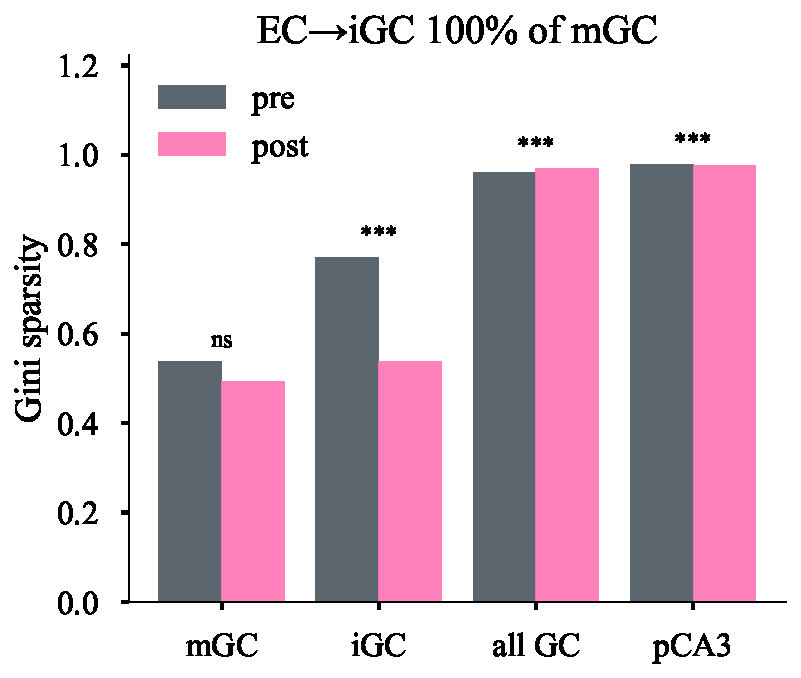
\includegraphics[width=0.31\textwidth]{figures/supplementary/opto_sparsity_neurogenesis_1.0.pdf}\hfill
    \hspace{0.31\textwidth}\hfill
    \hspace{0.31\textwidth}%
\label{fig:opto_sparsity}
\end{figure}

\clearpage
\begin{figure}[H]
    \centering
    \caption{Rhythmicity of the post-pulse response of each population. Left column, population firing rate over the
        \SIrange{5}{60}{\milli\second} window following the onset of the depolarizing pulse delivered to half of the iGCs, pooled
        over all EC$\to$iGC connection probabilities and all runs. Right column, power spectrum of the same signal after
        subtraction of a Gaussian-smoothed envelope, estimated by Welch's method over the \SIrange{20}{200}{\hertz} band; the
        dashed line and the label mark the peak frequency. Only the BCs show a spectral peak that stands out from the background
        of their own spectrum, at the frequency reported in the Results chapter; the peak of the MCs carries a power close to the
        median of their band and the remaining populations peak at the lower edge of the band. The \SI{55}{\milli\second}
        analysis window sets the frequency resolution at \SI{18}{\hertz}, so the peak frequencies are accurate only to within one
        bin.}

    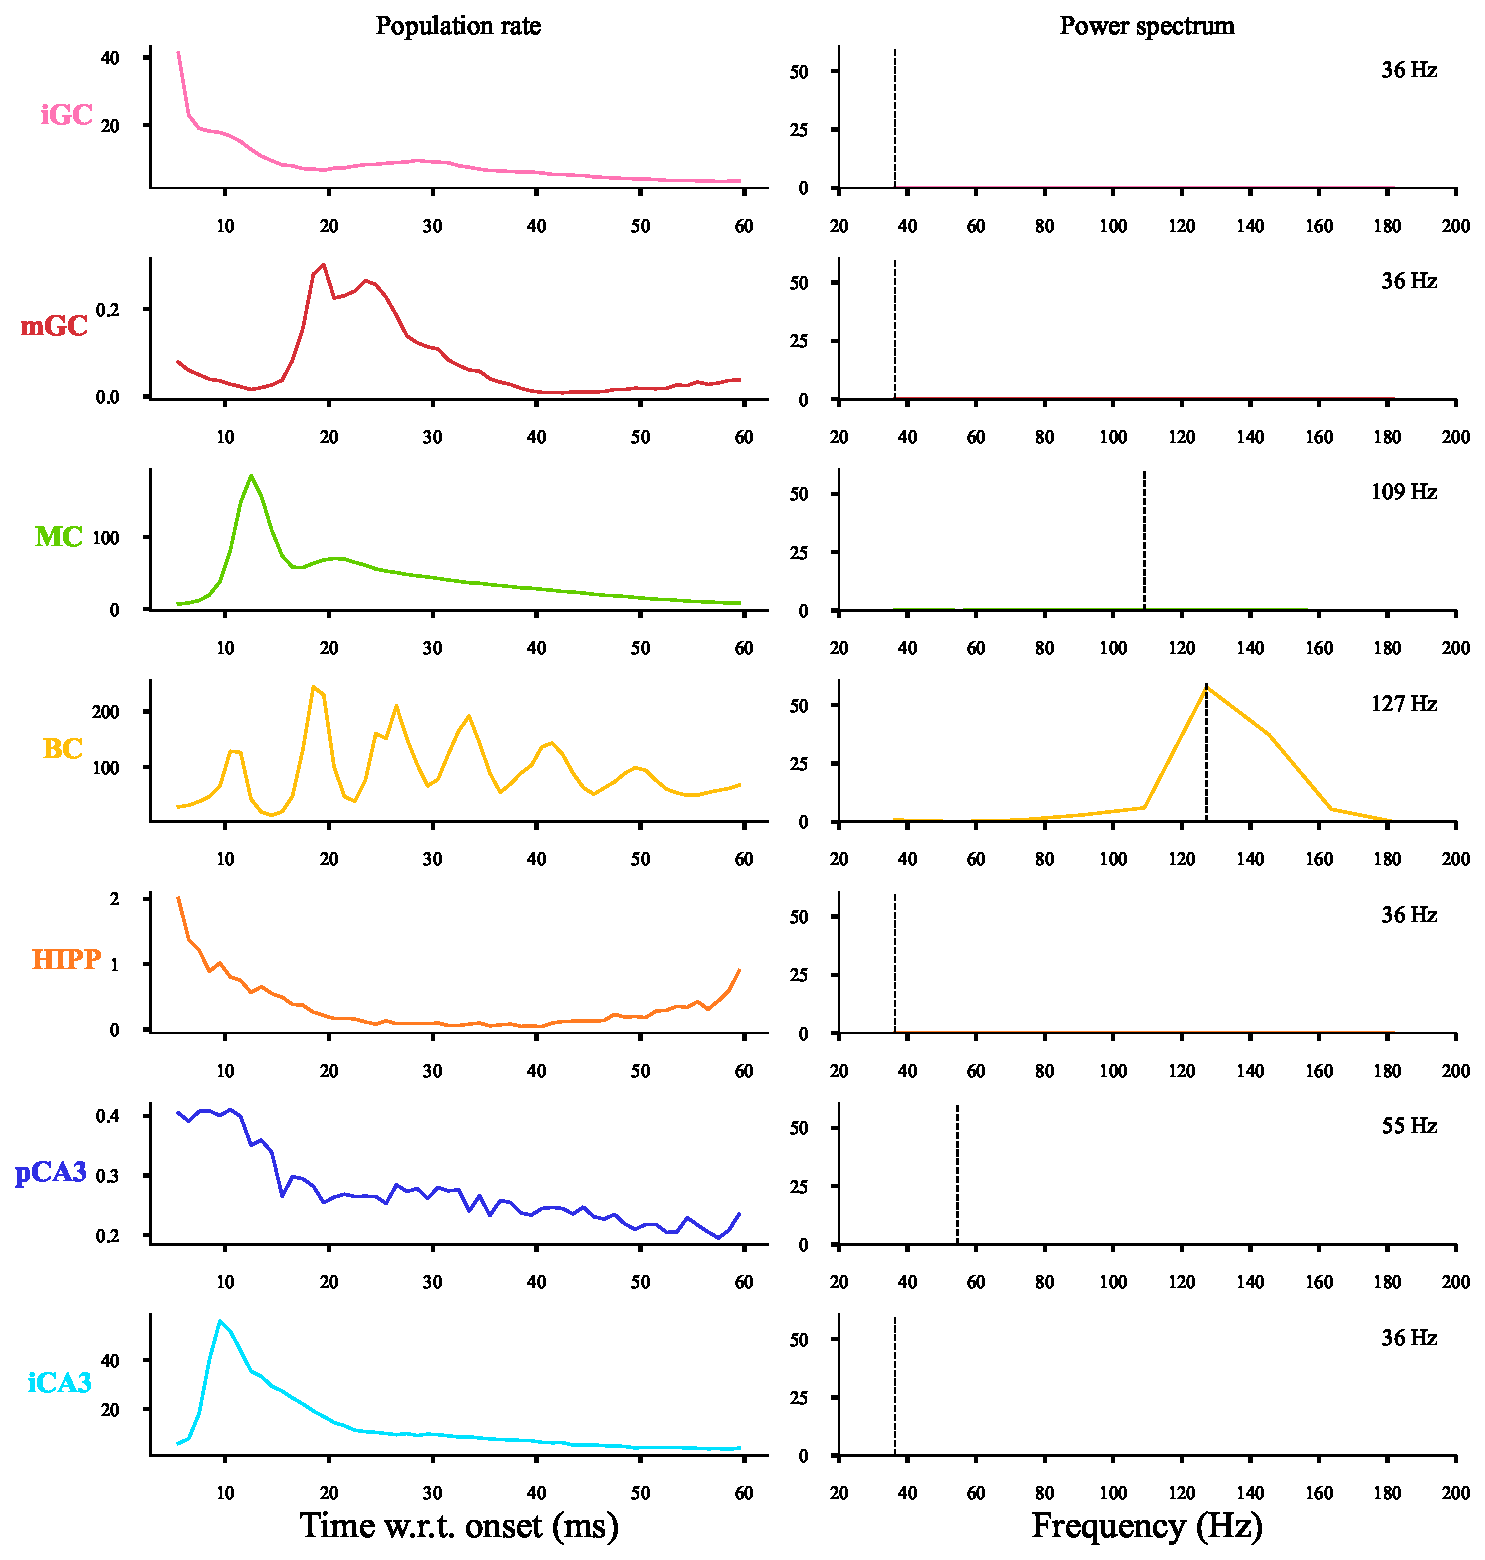
\includegraphics[width=0.9\textwidth]{figures/supplementary/frequency_pos_all.pdf}%
\label{fig:frequency_spectra}
\end{figure}

\end{apendicesenv}
